\documentclass[12pt,a4paper]{scrartcl}
\usepackage[latin1]{inputenc}
\usepackage{amsmath}
\usepackage{amsfonts}
\usepackage{amssymb}
\usepackage{graphicx}
\author{Christian Neuberger}
\title{R\_Visualizer Manual}

\usepackage[hidelinks,colorlinks=false]{hyperref}
\usepackage{placeins}
\usepackage{wrapfig}

\newcommand*{\fullref}[1]{\hyperref[{#1}]{\autoref*{#1} \nameref*{#1}}} % One single link

\begin{document}

\maketitle
\newpage

\tableofcontents
\newpage

\section{About R\_Visualizer}
\label{sec:About}
R\_Visualizer is a graphical tool used to observe and control the state of a compatible system. Said system is connected to the host pc running R\_Visualizer via the CAN-Analyser USB interface. This interface will continually receive CAN messages from the system and propagate these messages to R\_Visualizer and vice versa. Received messages will subsequently be visualized by R\_Visualizer. The application itself is capable of sending messages to the system via the CAN-Analyser USB interface to control the system state or behavior.

\section{Installing}
\label{sec:Installing}
There is no installation needed. Simply unzip the provided zip file to any location you desire that does not require administrative priviledges and start the application via the \textit{R\_Visualizer.exe} file. Do not delete any file or folder from the unzipped folder.

\section{Getting Started}
\label{sec:GettingStarted}

This section will guide you through R\_Visualizer and show you how to use the basic functionalities of the Application.
\begin{itemize}
	\item For a quick Overview refer to \fullref{subsec:GettingStartedOverview} 
%	\item For a quick Setup refer to \fullref{subsec:GettingStartedSetup}
	\item For a quick Connecting to to the system guide refer to \fullref{subsec:GettingStartedEstablishConnection}
	\item For a quick Quickstart guide refer to \fullref{subsec:GettingStartedQuickStart}
\end{itemize}

\subsection{Overview}
\label{subsec:GettingStartedOverview}
The general user interface is designed with simplicity in mind. The main goal was to expose as much information as possible without distracting the user with cluttered configuration dialogs. Therefore, the interface is divided into two main parts: the message stream on the left-hand side and the overview/configuration dialogs on the right-hand side. 

Most of the application is tailored to the current user. A user can either be a regular user or an \textit{Admin}. The regular user is only exposed to basic functionality that is needed to monitor and control the observed system. On the other hand, the \textit{Admin} user has advanced functionality like storing or editing configuration entries. The user roles can be switched with the respective symbol in the shortcut panel or from the \textit{User} menu at the top of the application.

\FloatBarrier
\subsubsection{Menu}
\label{subsubsec:GettingStartedOverviewMenu}
The \textit{Menu} is comprised of the items: 

\begin{itemize}
\item File (see \fullref{fig:menuFile})\\
can be used to load a recent \textit{Message Stream} or store the current \textit{Message Stream}. Additionally, the \textit{Error Log} is accessible from the \textit{File} menu.\footnote{Currently the \textit{New} option is used for testing. It does not flush the \textit{Message Stream} to create a new stream but rather adds example messages to the stream...}
\begin{itemize}
	\item New - TESTING ONLY
	\item Open - Open a previously saved \textit{Message Stream}
	\item Save - Save the current \textit{Message Stream}
	\item Show Error Log - Displays the current \textit{Error Log}\footnote{ONLY CAN errors are displayed here.}
\end{itemize}
\item Trace (see \fullref{fig:menuTrace})\\
can be used to establish a connection to the CAN-Analyser USB interface and to disconnect R\_Visualizer from the CAN-Anylser USB interface, as well as starting and stopping the recording of messages.\footnote{Keep in mind that stopping the message recording will stop the Message Stream from storing incoming messages. Messages that are not stored by the Message Stream are lost and cannot be retrieved by any means.}
\begin{itemize}
	\item (Dis)Connect - Connect or disconnect to the CAN-Analyser USB interface\footnote{The functionality of the menu entry depends on the current connection state.}
	\item Start - Start recording incoming messages to the \textit{Message Stream}(Connect first!)
	\item Stop - Stop recording incoming messages to the \textit{Message Stream}
\end{itemize}
\item User (see \fullref{fig:menuUser})\\
can be used to switch between \textit{Admin} and \textit{User} mode.
\begin{itemize}
	\item Admin/User - Switch to the currently displayed user role
\end{itemize}
\end{itemize}

All items from all sub-menus can also be accessed through the respective shortcut buttons in the menu panel.

\begin{figure}
	\centering
	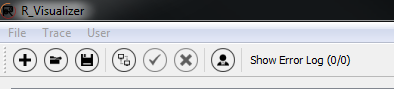
\includegraphics[width=0.7\linewidth,keepaspectratio]{Graphics/Menu}
	\caption[Menu]{}
	\label{fig:menu}
\end{figure}
\begin{figure}
	\centering
	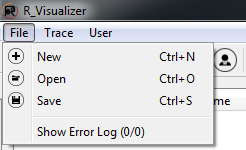
\includegraphics[width=0.55\linewidth,keepaspectratio]{Graphics/MenuFile}
	\caption[File Menu]{}
	\label{fig:menuFile}
\end{figure}
\begin{figure}
	\centering
	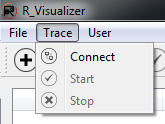
\includegraphics[width=0.5\linewidth,keepaspectratio]{Graphics/MenuTrace}
	\caption[Trace Menu]{}
	\label{fig:menuTrace}
\end{figure}
\begin{figure}
	\centering
	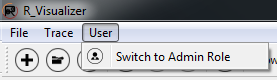
\includegraphics[width=0.6\linewidth,keepaspectratio]{Graphics/MenuUser}
	\caption[User Menu]{}
	\label{fig:menuUser}
\end{figure}


\FloatBarrier
\subsubsection{Message Stream}
\label{subsubsec:GettingStartedOverviewMsgStream}

\begin{wrapfigure}{r}{0.6\textwidth}
	\centering
	\vspace{-0.5cm}
	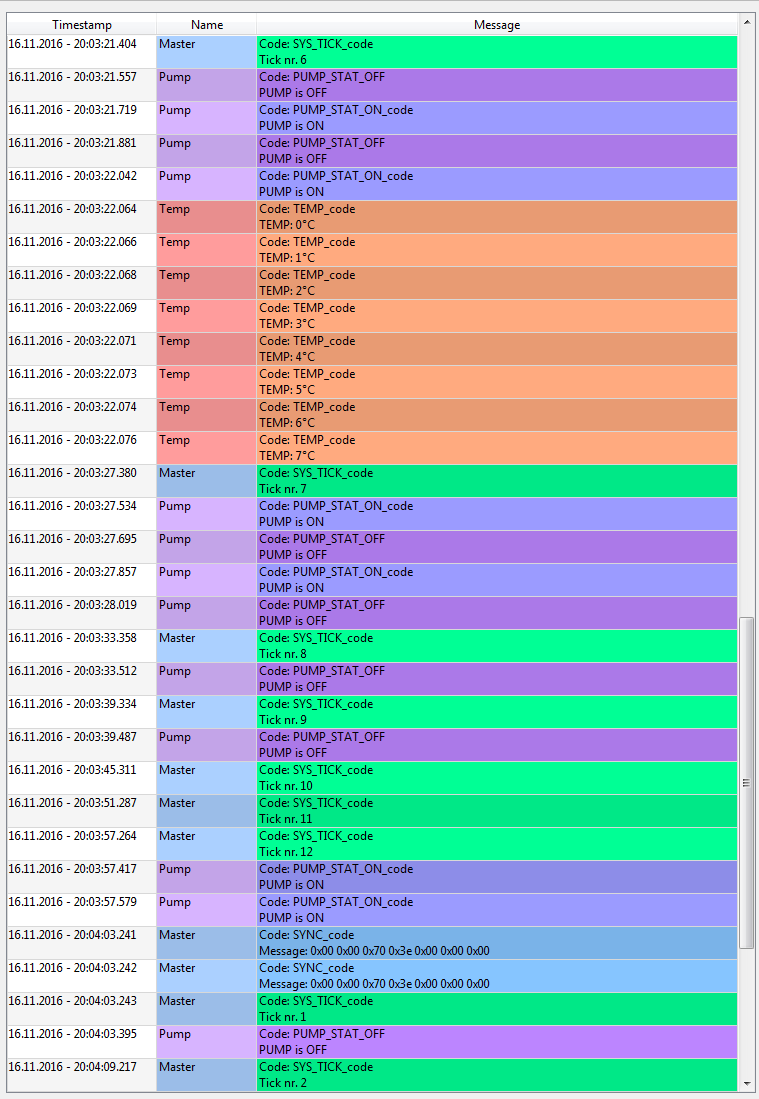
\includegraphics[width=0.55\textwidth,keepaspectratio]{Graphics/MessageStream}
	\caption[Message Stream]{The \textit{Message Stream} displaying incoming messages}
	\label{fig:MessageStreamOvrv}
\end{wrapfigure}

To achieve maximum exposure of the system behavior, the \textit{Message Stream} is visible in all configuration dialogs and during the system overview dialog. The incoming messages are continuously updated and displayed. 

The \textit{Message Stream} displays messages in the order they are picked up by the CAN-Anylser USB interface: in a chronological order. The messages visualization is customizable via the configuration dialogs in the \textit{Message Config} tab (see \fullref{fig:MessageStreamOvrv}). Per default messages are displayed with their respective timestamp, id and code plus data. 

The user can use scrolling to view any messages that were picked up by the \textit{Messages Stream}, there is no limitation on the history.

\FloatBarrier
\clearpage

\subsubsection{System Overview}
\label{subsubsec:GettingStartedOverviewSysOverview}
\textbf{CURRENTLY NOT IN A PRODUCTION STATE. USE AT OWN RISK.}

The System Overview tab can be used to visually recreate the connected system and observe the system's current state.

\FloatBarrier
\subsubsection{Send Messages}
\label{subsubsec:GettingStartedOverviewSendMsgs}
In order to communicate and control the system, the \textit{Send Messages} tab provides the means to send single messages or whole packages of messages to the system (see \fullref{fig:SendMessagesOvrv})

\begin{wrapfigure}{r}{0.6\linewidth}
	\centering
	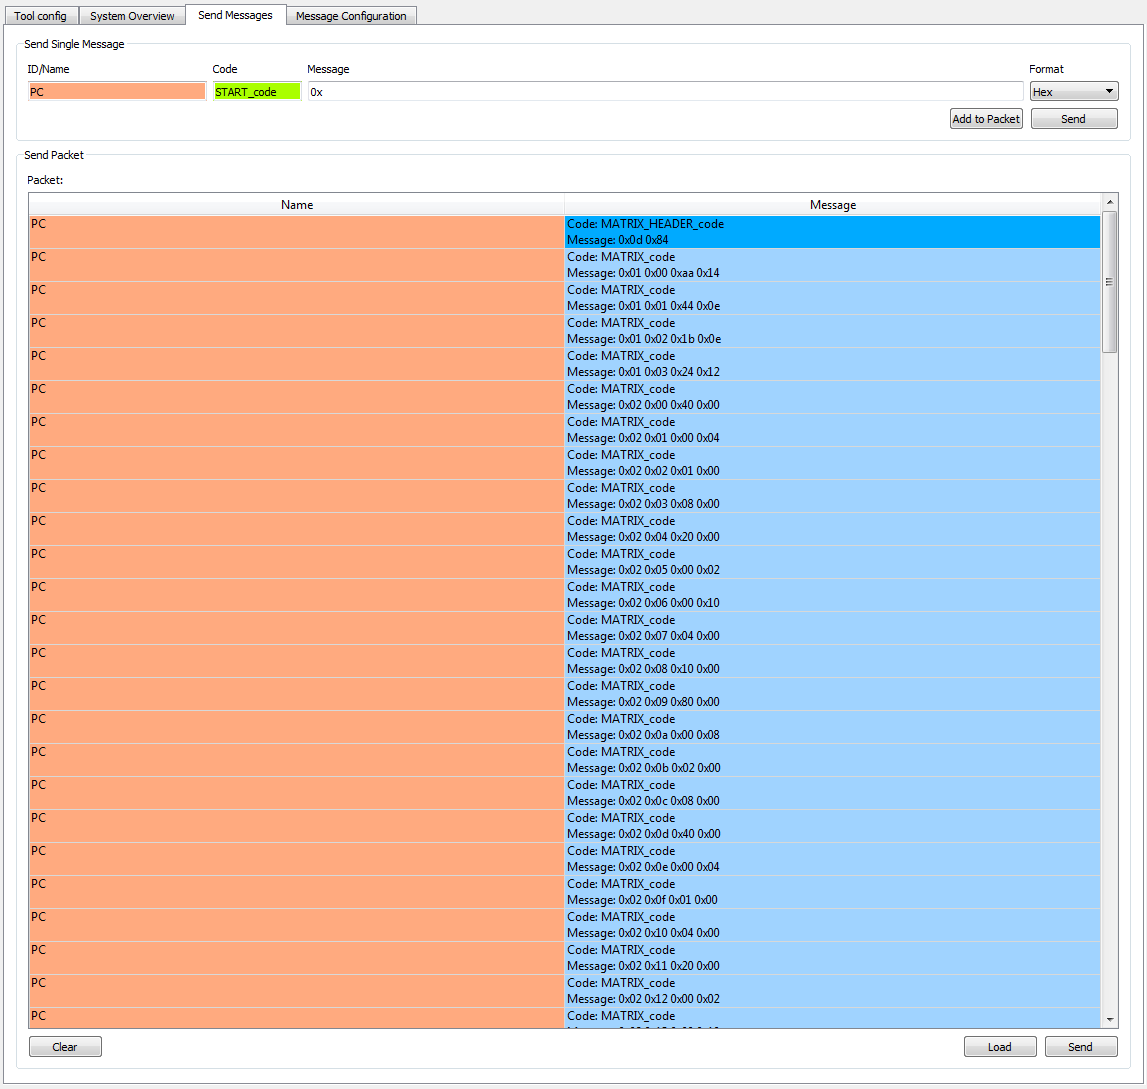
\includegraphics[width=\linewidth,keepaspectratio]{Graphics/SendMessagesOverview}
	\caption[Send Messages Dialog]{The \textit{Send Messages} dialog that can be used to send single messages or whole packages of messages in the specified order}
	\label{fig:SendMessagesOvrv}
\end{wrapfigure}

\paragraph{Sending single messages} can be achieved with the Send Single Message sub-dialog within the \textit{Send Messages} tab. Type in an ID that shall be exposed to the system as the sender of the message, the desired code to send and additionally the data you want to send with the message. 

The ID/Name field can be filled with a numerical value in decimal or hexademical format\footnote{for hexadecimal prepend 0x to the hexadecimal number}. If the ID to name mapping has already been loaded or created in the \textit{Message Config} tab, it is also possible to type in the specified name or choose one from the auto-completion list.

The Code field can be filled with a numerical value in decimal or hexademical format\footnote{for hexadecimal prepend 0x to the hexadecimal number}. If the Code to name mapping has already been loaded or created in the \textit{Message Config} tab, it is also possible to type in the specified name or choose one from the auto-completion list. 

The Data field can be filled with numerical values according to your selection in the the combo box right next to the data field. The application will translate the entered data to an internal byte-wise representation automatically.
The specific data format can be one of the following:

\begin{itemize}
\item Hex\\
hex values in portions of bytes
\item Dec Data\\
decimal values in portions of bytes\footnote{Keep in mind that one byte must not exceed the number 255}
\item Dec Value\\
one decimal value which will automatically be translated to bytes by the application\footnote{Keep in mind not to exceed the 56bit limitation, which is 72057594037927935}
\item Bin\\
binary values (byte-wise)
\end{itemize}

When switching the selection of the combo box the value is automatically translated from the last selection to the new selection\footnote{Keep in mind that translating from a value-based notation to a byte-wise notation or vice versa might mess up the byte order.}

\paragraph{Sending packages of messages} can be achieved with the \textit{Send Packet} sub-dialog in the \textit{Send Messages} tab. In order to load a matrice of messages, simply click load and select the desired matrix to load in either .csv or .json format\footnote{The .json format is kept to comply with the rest of the application's data. Only load .json files that were previously saved with the Send Packet Store function.}. To Send the whole package of messages in a chronological order from top to bottom simply click on Send. To clear the current Packet click on the Clear button. It is not necessary to clear the view before loading another Packet. The display style of the loaded message packet is similar to the \textit{Message Stream's} display style, because both entities rely on the same \textit{ID} and \textit{Message Type} configuration.

\FloatBarrier
\subsubsection{Message Configuration}
\label{subsubsec:GettingStartedOverviewMsgConfig}
The \textit{Message Configuration} tab directly interferes with the \textit{Message Stream}. It consists of three separate sub-dialogs: Filter, IDs and Message Types (see \fullref{fig:MessageConfigOvrv})

\begin{figure}
	\centering
	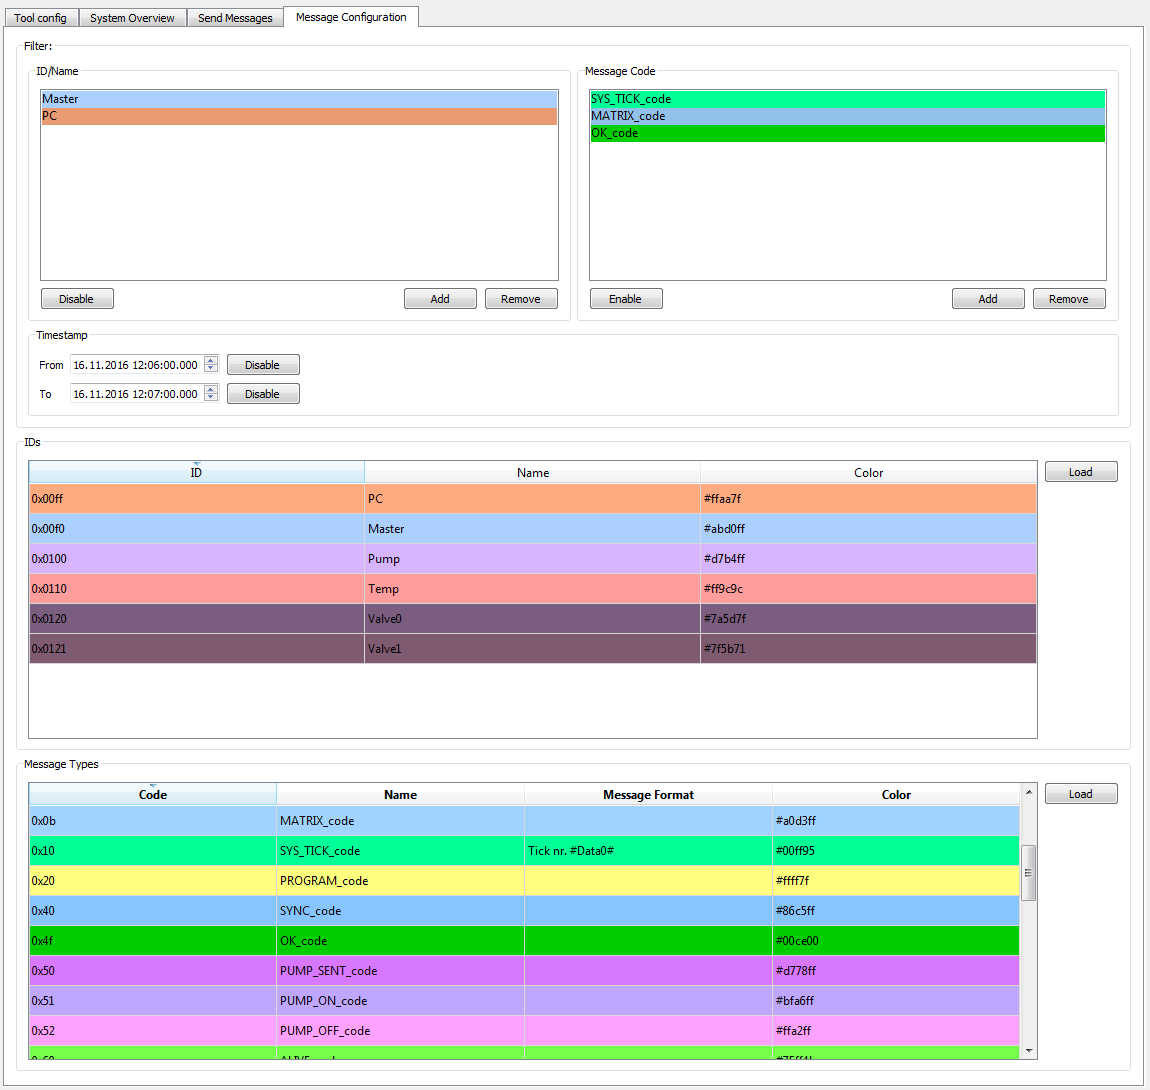
\includegraphics[width=\linewidth,keepaspectratio]{Graphics/MessageConfigOverview}
	\caption[Message Configuration Dialog]{The \textit{Message Configuration} dialog that can be used to enhance the visual representation of messages in the \textit{Message Stream} and to filter for specific messages in the \textit{Message Stream}}
	\label{fig:MessageConfigOvrv}
\end{figure}

\FloatBarrier

\paragraph{The Filter section} can be used to filter the \textit{Message Stream} for certain properties (see \fullref{fig:MessageConfigFilter}). The filters are chained. To be more specific, the filters interact with each other to display only messages that suffice all enabled filter criteria at onces. Use multiple filters to get a fine-grained filtering of the \textit{Message Stream}. Since the \textit{Messages Stream} is updated live, it is advised to first setup all of the desired filter criteria and then enable all filters, starting from the most general one.

\begin{figure}
	\centering
	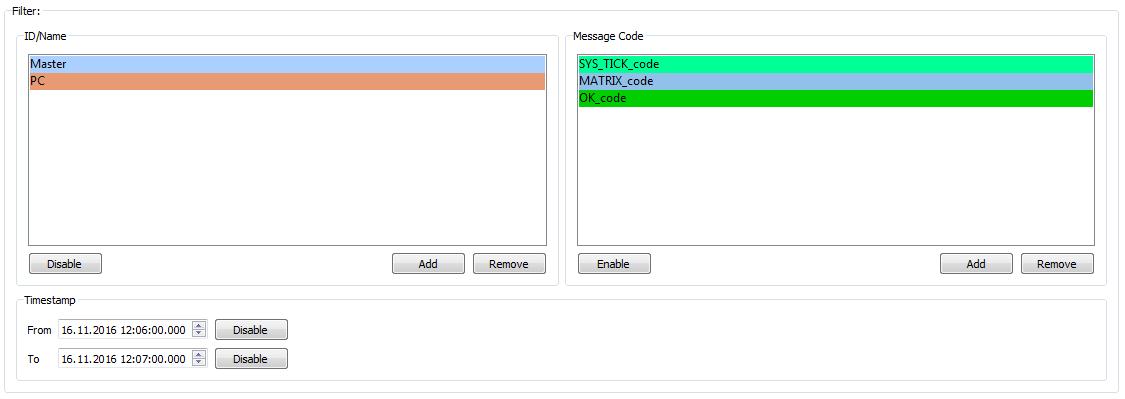
\includegraphics[width=0.8\linewidth,keepaspectratio]{Graphics/MessageConfigFilter}
	\caption[Message Configuration Filter]{The \textit{Message Configuration} Filters that can be used to filter the \textit{Message Stream} for specific messages}
	\label{fig:MessageConfigFilter}
\end{figure}

\subparagraph{The ID/Name subsection} can be used to filter for certain IDs or -provided the ID to name mapping has been setup appropriately- names. To create an ID filter, simply click the \textit{Add} button and type in the desired ID in either decimal or hexadecimal representation\footnote{for hexadecimal prepend 0x to the hexadecimal number}. If and only if an ID to name mapping has been set up, the respective names can be entered directly or chosen from the auto-completion dialog. To remove a filter, select the according entry from the list and click on the \textit{Remove} button. Per default the ID/Name filter is disabled. To enable the filter click on the \textit{Enable} button.\footnote{It is advised to first add all desired filter criteria before enabling the filter, because the \textit{Message Stream} will be updated with each new entry which leads to increased workload}.

\subparagraph{The Code subsection} can be used to filter for certain code or -provided the code to name mapping has been setup appropriately- names. To create a code filter, simply click the \textit{Add} button and type in the desired Code in either decimal or hexadecimal representation\footnote{for hexadecimal prepend 0x to the hexadecimal number}. If and only if a code to name mapping has been set up, the respective names can be entered directly or chosen from the auto-completion dialog. To remove a filter, select the according entry from the list and click on the \textit{Remove} button. Per default the Code/Name filter is disabled. To enable the filter click on the \textit{Enable} button.\footnote{It is advised to first add all desired filter criteria before enabling the filter, because the \textit{Message Stream} will be updated with each new entry which leads to increased workload}.

\subparagraph{The Timestamp subsection} can be used to filter for a certain period of time. Both, the \textit{from} as well as the \textit{to}, can be enabled or disabled independently from another. Setting the \textit{from} parameter will automatically adjust the \textit{to} parameter and vice versa to form a meaningful time span -even if disabled. Again, it is advised to adjust the parameters with the filters being disabled in order to gain performance.

\FloatBarrier
\paragraph{The IDs section} can be used to alter the visualization of the \textit{Message Stream's} \textit{Name} column (see \fullref{fig:MessageConfigIDs}). Each ID can be assigned to an alias and a color. If a message in the \textit{Message Stream} matches against a configured ID, its name will be displayed instead of the numerical representation and the respective field will be colored in the configured color. This is especially useful to rapidly distinguish different message senders in the \textit{Message Stream}. In addition, all fields in all other menus that require IDs are updated to auto-complete if a name to a configured ID is entered. Most of the fields are then also colored respectively.

\begin{figure}
	\centering
	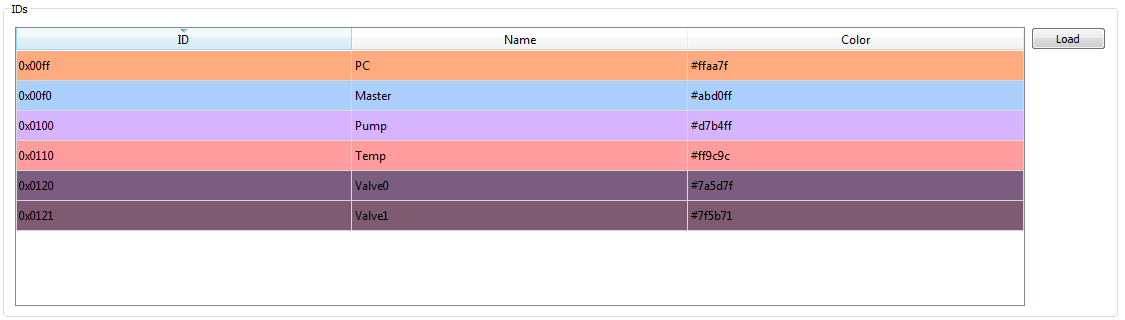
\includegraphics[width=\linewidth,keepaspectratio]{Graphics/MessageConfigIDs}
	\caption[Message Configuration IDs]{The \textit{Message Configuration} IDs that can be used to set alias name and coloring for the \textit{Message Stream's} Name column}
	\label{fig:MessageConfigIDs}
\end{figure}

\FloatBarrier
\paragraph{The Message Types section} can be used to alter the visualization of the \textit{Message Stream's} \textit{Message} column (see \fullref{fig:MessageConfigMessageTypes}). Each Code can be assigned to an alias and a color. In addition, a message format can be set with the message formatter dialog that will be used to parse the data portion and code of an incoming message to a visually appealing format. If a message in the \textit{Message Stream} matches against a configured Code, its name will be displayed instead of the numerical representation and the respective field will be colored in the configured color. In addition, the configured message format will be used to enhance the representation of the message. This is especially useful to rapidly distinguish different messages by code in the \textit{Message Stream}. In addition, all fields in all other menus that require Codes are updated to auto-complete if a name to a configured Code is entered. Most of the fields are then also colored respectively.

\begin{figure}
	\centering
	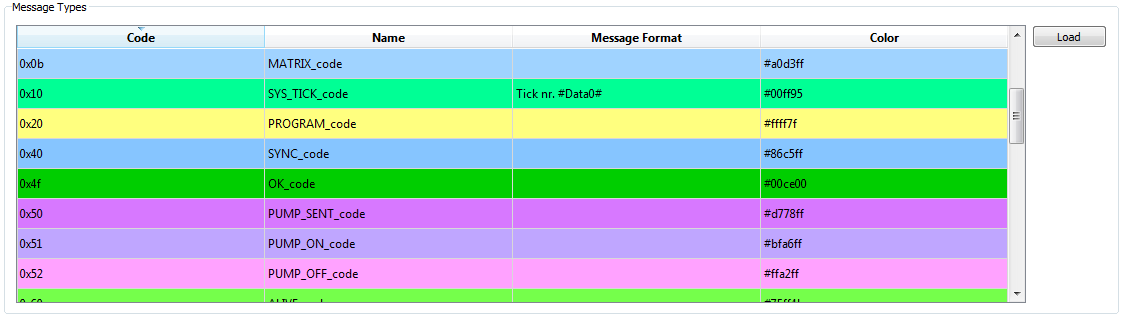
\includegraphics[width=\linewidth,keepaspectratio]{Graphics/MessageConfigMessageTypes}
	\caption[Message Configuration Message Types]{The \textit{Message Configuration} Message Types that can be used to set alias name and coloring for the \textit{Message Stream's} Message column and format the messages' data}
	\label{fig:MessageConfigMessageTypes}
\end{figure}

\FloatBarrier
%\subsection{Setting up R\_Visualizer}
%\label{subsec:GettingStartedSetup}


\FloatBarrier
\subsection{Connecting the Host PC to the System}
\label{subsec:GettingStartedEstablishConnection}
The CAN-Analyser USB interface has exactly two outputs: a standard USB connector and a four pin CAN connector. The CAN connector shall be connected to the observed System's CAN bus, whereas the USB connector shall be connected to the host PC.

\subsubsection{Connection to the System}
\label{subsubsec:GettingStartedEstablishConnectionConnectionToSystem}
Make sure that the system is not powered\footnote{Sidenote: It is possible to plug in the CAN-Analyser USB interface while the system is powered on (or even running), but it is not advised. System failure or damage could be the result.}. Connect the CAN-Analyser USB interface to one of the free connectors on the system's CAN bus using a supplied CAN compatible cable. 


\subsubsection{Connection to the Host PC}
\label{subsubsec:GettingStartedEstablishConnectionConnectionToHost}
Simply plug the CAN-Analyser USB interface into one of your host PC's USB ports\footnote{Either USB 2 or USB 3; both are supported.}. Windows should be able to deduct the needed driver and install the CAN-Analyser USB interface accordingly. 

The drivers needed are the HID driver and a USB driver. When the host PC is equipped with either a keyboard, a mouse or any other kind of standard input device, the HID driver should be pre-installed. When the host PC is equipped with USB ports, the USB drivers should be pre-installed. 

It is advised to use a USB extension cable. Since the CAN-Anylser USB interface is moderately sized and only held by the USB connector, the USB connector can easily be destroyed by force in either direction when applied to the plugged in CAN-Analyser USB interface. Moreover, the whole CAN-Analyser USB interface might take damage when exposed to force.

Additionally it is advised to plug the CAN-Analyser USB interface into a self-powering USB hub in order not to damager the host PC's USB ports in case of unexpected system failure. This scenario is quite unrealistic, since the CAN-Analyser USB interface has been tested thoroughly, but worthing noting.


\FloatBarrier
\subsection{Quickstart Guide}
\label{subsec:GettingStartedQuickStart}
In order to test the application's functionality follow these steps to set up R\_Visualizer quickly with some example data. This guide is intended to display the capabilities and mechanisms. Since this guide will only focus on loading, displaying and configuring already existent data, the steps needed to connect to a real system are left out. For further details on interaction with a real system please refer to  \fullref{sec:Observing}.\\

\textbf{Quickstart:}
\begin{itemize}
	\item Navigate to the application directory using either the explorer or a command line
	\item Start the Application by starting \textit{R\_Visualizer.exe}\\
	$\rightarrow$ R\_Visualizer starts and displays its main screen
	\item Open the already prepared test \textit{Message Stream} by either using the \textit{File} menu, the respective shortcut button in the menu panel or by using the shortcut \textit{ctrl+o}
	\begin{itemize}
	\item In the opening dialog navigate to the \textit{TestData} directory and open \textit{TestRun.json}
	\item R\_Visualizer will now load an example \textit{Message Stream} that was recorded by R\_Visualizer earlier
	\end{itemize}
	\item To customize the appearance of the \textit{Message Stream}, navigate to the \textit{Message Configuration} to on the right-hand side of the main window
	\begin{itemize}
		\item To enhance the visual appearance of the \textit{Message Stream's} Name column, load an \textit{IDs} File by clicking on \textit{Load} in the \textit{IDs} subsection
		\begin{itemize}
			\item In the \textit{TestData} directory you will be able to locate an \textit{IDs.json} file.
			\item Open said file and R\_Visualizer will automatically populate the IDs subsection with the data contained in the file
			\item If successful the \textit{Message Stream} will update immediately to display the enhanced Name column
		\end{itemize}
		\item To enhance the visual appearance of the \textit{Message Stream's} Message column, load an \textit{Message Types} File by clicking on \textit{Load} in the \textit{Message Types} subsection
		\begin{itemize}
			\item In the \textit{TestData} directory you will be able to locate an \textit{MessageTypes.json} file.
			\item Open said file and R\_Visualizer will automatically populate the Message Types subsection with the data contained in the file
			\item If successful the \textit{Message Stream} will update immediately to display the enhanced Message column
		\end{itemize}
	\end{itemize}
	\item Feel free to browse through the \textit{Message Stream}
	\item To filter the \textit{Message Stream}, navigate to the \textit{Message Configuration} tab on the right-hand side of the main screen
	\begin{itemize}
		\item To filter for certain IDs/Names use the \textit{ID/Name} subsection of the Filter section
		\begin{itemize}
			\item To add an ID/Name filter criteria click on the Add button
			\item You will now be prompted to enter the ID/Name to filter
			\item Since you have already loaded an \textit{IDs} file, you can now enter the Name to filter for or the numerical representation in either decimal or hexadecimal
			\item Finally enable filtering for your ID/Name filter criteria by clicking on Enable
		\end{itemize}
		\item To filter for certain Message Codes use the \textit{Message Code} subsection of the Filter section
		\begin{itemize}
			\item To add a Message Code filter criteria click on the Add button
			\item You will now be prompted to enter the Code/Name to filter
			\item Since you have already loaded an \textit{Message Types} file, you can now enter the Name to filter for or the numerical representation in either decimal or hexadecimal
			\item Finally enable filtering for your Message Code filter criteria by clicking on Enable
		\end{itemize}
		\item To filter for a certain timespan use the \textit{Timestamp} subsection of the Filter section
		\begin{itemize}
			\item To only display messages that were recorded after a certain point in time edit the From field of the Timestamp subsection
			\item To only  display messages that were recorded before a certain point in time edit the To field of the Timestamp subsection
			\item Enable the respective Timestamp filter by clicking on the respective Enable button
			\item Both Timestamp filters can be combined by enabling both Timestamp filters in order to filer for a certain timespan
		\end{itemize}
	\end{itemize}
	\item To close R\_Visualizer simply click on the X in the top right corner, use the shortcut \textit{alt+F4} or any other preferred method of closing windows applications.
\end{itemize}


\FloatBarrier
\section{Observing a System}
\label{sec:Observing}
In order to observe a system, first connect the system via the CAN-Analyser USB interface to the host PC as described in \fullref{subsec:GettingStartedEstablishConnection}. After connecting the interface to the host PC establish a connection between R\_Visualizer and the interface by clicking on the connect symbol in the menu panel or selecting the respective entry from the \textit{Trace} menu. If the connection is established successfully the \textit{Connect} symbol changes to the \textit{Disconnect} symbol. If the connection cannot be established you are prompted to connect the CAN-Anylser USB interface to the host PC correctly. Given a connection has been established start recording incoming messages by clicking on the Start symbol in the menu panel or selecting Start from the trace menu. If the recording has started successfully the Start symbol will be greyed out and the Stop symbol will be activated.

As soon as the recording is started the \textit{Message Stream} is updated with each new incoming message. All incoming messages are stored in the application and can be viewed using the \textit{Message Stream}.

The Message Stream visualization can be configured using the Message Configuration tab as described in \fullref{subsubsec:GettingStartedOverviewMsgConfig}.

\FloatBarrier
\section{Inspecting the Aggregated Data}
\label{sec:Inspecting}
A currently recorded \textit{Message Stream} can be saved to disk by clicking on the Save shortcut in the menu panel or selecting Save from the File menu. At any time a \textit{Message Stream} can be loaded by clicking on the Open shortcut in the menu panel or selecting Open from the File menu. It is advised to stop and save a currently active recording before opening a new \textit{Message Stream}, because the current stream will be flushed and the data is lost if not saved. New incoming messages will be appended to the loaded \textit{Message Stream}.

All configurations made in the \textit{Message Configuration} tab are applied to the current \textit{Message Stream}. Use filters to narrow the displayed data to a desired result.

\FloatBarrier
\section{Controlling a System}
\label{sec:Controlling}
If and only if a connection to the system has been established correctly (see \fullref{sec:Observing}), it is possible to directly interact with the system by sending single messages or whole packages of messages to the system.

To send single messages use the \textit{Send Single Message} sub-dialog in the \textit{Send Messages} tab. The ID/Name that will be used to indicate the sender of the message can be entered into the ID/Name field. It is possible for the R\_Visualizer application to be seen as any node in the system from the system's point of view. This is especially useful when testing new functionalities or provoking abnormal system behavior\footnote{USE WITH CAUTION!}. Usually the ID/Name to be entered here is the one of the host PC, in oder to appear as the PC node to the system.

To send a control matrix, load the corresponding matrix into the \textit{Send Packet} sub-dialog by clicking Load underneath the Packet visualization. A loaded matrix will be displayed in the Packet visualization upon loading. To send the loaded matrix click on \textit{Send}, which will then instruct R\_Visualizer to send the matrix with the given messages to the system chronologically starting from the first entry.

It is possible to construct a new package by entering the desired message into the Send Single Message sub-dialog and clicking on \textit{Add to Packet}. This will append a new message with the given fields to the current message package. In order to clear a previously loaded message package (e.g. to construct a new one, click on \textit{Clear}).

\FloatBarrier
\newpage
\listoffigures

\end{document}